% Example LaTeX document for GP111 - note % sign indicates a comment
\documentclass[12pt,a4paper,oneside]{article}
\usepackage{lmodern}
\usepackage[french]{babel}
\usepackage[T1]{fontenc}
\usepackage[utf8]{inputenc}
\usepackage{graphicx}
\usepackage{hyperref}
\usepackage{float}
\usepackage[ruled,vlined]{algorithm2e}
\usepackage[backend=bibtex,style=verbose-trad2,natbib=true]{biblatex}
\graphicspath{{../images/}}
\usepackage{ccaption}

% Default margins are too wide all the way around. I reset them here
\setlength{\topmargin}{-.5in}
\setlength{\textheight}{9in}
\setlength{\oddsidemargin}{.125in}
\setlength{\textwidth}{6.25in}

\hypersetup{
    unicode=false,          % non-Latin characters in Acrobat’s bookmarks
    pdftoolbar=true,        % show Acrobat’s toolbar?
    pdfmenubar=true,        % show Acrobat’s menu?
    pdffitwindow=false,     % window fit to page when opened
    pdfnewwindow=true,      % links in new window
    colorlinks=true,       % false: boxed links; true: colored links
    linkcolor=black,          % color of internal links (change box color with linkbordercolor)
    citecolor=green,        % color of links to bibliography
    filecolor=magenta,      % color of file links
    urlcolor=cyan,          % color of external links
    linktoc=page
}

\begin{document}

\begin{titlepage}
\begin{flushright}
           
\includegraphics[scale=0.30]{../images/univorleans.png}\\ 
                      Département Informatique
\end{flushright}
\vspace{20mm}
\begin{center}
\textbf{\huge{Documentation Technique}}\\
\vspace{20mm}
\begin{large}
	\textit{Zo RABARIJAONA}\\
	\textit{Jérémy MOROSI}\\
	\textit{Willy FRANÇOIS}\\
	\textit{Raya DJADLI}
\end{large}

\end{center}
\begin{figure}[b!]
\begin{flushright}
~~\\ ~~\\ ~~\\ ~~\\ ~~\\ ~~\\ ~~\\
\large{Année : 2013-2014}
\end{flushright}
\end{figure}
\end{titlepage}

\newpage

\tableofcontents

\newpage

\section{Analyse}


\subsection{Des applications difficilement modifiables}

Castle Defense, librarie, code natif, attaque héxa, rétro engeneering...


\subsection{L'Application Checkers}

l'application Checkers (principe), décompilation, un bytecode obscure
dex2jar, jd-gui, correction des erreurs, éclaircissement du code, une archi mvc.
Fonctionnement de l'appli en interne
\subsubsection{Principe}
\begin{figure}[hp]
	      \begin{center}
		\fbox{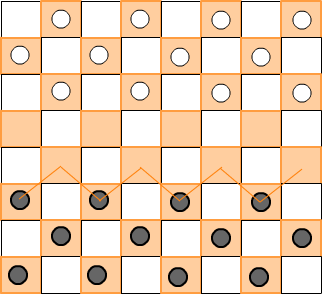
\includegraphics[scale=0.5]{principe}}
	      \end{center}
	\legend{Principe}
\end{figure}
Le jeu est composé de 8 cases sur 8, c’est-à-dire 4 cases en moins que le jeu de dame classique.  Se joue en deux modes : utilisateur contre ordinateur ou utilisateur contre utilisateur.\\
Un joueur peut choisir une couleur (des pions/dames noires ou des pions/dames blanche).  Le jeu est initialement constitué de 3 lignes de 4 pions espacés d’une case. Chaque pion/dame peut se déplacer en diagonale. 
Un pion se transforme en une dame (K) lorsqu’il arrive à la dernière ligne du camp de l’adversaire. Une dame ou un pion peut faire une prise en faisant un déplacement en diagonal. Mais une dame possède l’avantage de traverser plusieurs lignes vide.\\
Un joueur est désigné gagnant si l’adversaire ne possède plus de dames ou de pions.

\subsubsection{Décompilation et analyse du code}

Afin de pouvoir analyser le code de l'application plus aisément, nous avons dû trouver un moyen de décompiler l'application vers du code java.
Pour ce faire, nous avons utilisé \textit{dex2jar} \cite{dex2jar},
une api permettant de décompiler un fichier apk en un fichier jar contenant des fichiers class.
Ensuite, nous avons dû utiliser \textit{jd-gui} \cite{jdgui} sur ce fichier jar pour en afficher le code source.
L'application permet d'exporter les sources ainsi décompilées.

Une fois le code java de l'application en notre possession, nous avons pu commencer à l'analyser.
Nous avons vite remarqué que le code avait été obscurcit avant d'être compilé par le développeur de l'application.
Cela signifie que toutes variables et fonctions avaient un nom sans aucun sens, ce qui gêna la compréhension du code.
Nous avons aussi remarqué que la décompilation c'était mal passée à cause de return et de break à des endroits incongrus.
Nous avons donc commencé par supprimer ces erreurs afin de pouvoir avoir un code "compilable" sous Eclipse.
Ceci nous a offert un accès à l'outil de refactorisation de code pour renommer les variables après avoir compris à quoi elles pouvaient servir.

Malgré cela, à cause du problème de décompilation, certaines méthodes n'avaient aucun sens.
Nous avons donc décidé de relire le code smali des méthodes correspondantes afin de le traduire manuellement en java et ainsi avoir le code original exact.

\subsubsection{Architecture}
Dans un point de vue général, le développeur du jeu Checkers a adopté une architecture MVC. Ce qui nous a beaucoup aidé à determiner les différentes 
classes. 
\begin{figure}[hp]
	      \begin{center}
		\fbox{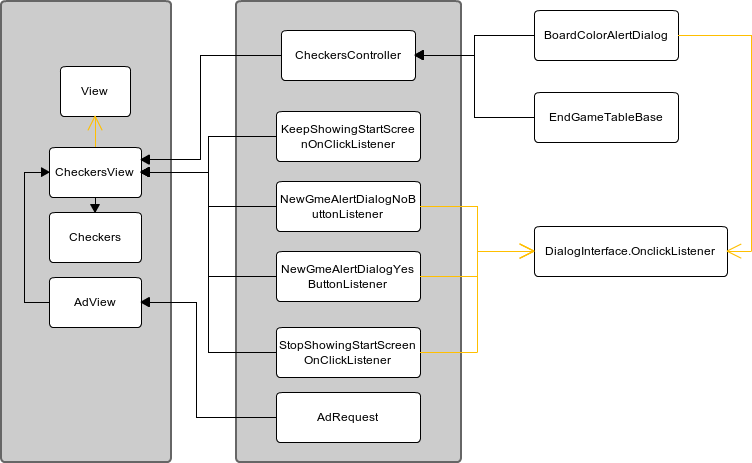
\includegraphics[scale=0.6]{archi}}
	      \end{center}
	\legend{architecture}
\end{figure}
La classe Checkers est la classe principale de l’application.
La classe CherckersView (b.smali) hérite de la classe android.view.View qui gére les vues de l’application. La classe AdView gère la vue pour la publicité.
CheckersController (a.smali) est le controleur principal de l’application. Les classes KeepShowingStartScreenOnclickListener (e.smali), NewGameAlertDialogNoButtonListener (d.smali), NewGameAlertDialogYesButtonListener (c.smali) et StopShowingStartScreenOnclickListener (f.smali) implémente l'interface DialogInterface.OnclickListener sont les classes qui gère les clics.
AdRequest est la classe qui est responsable du chargement de la publicité.


\section{Modifications apportées à l'Application}


\subsection{Ajout d'un bouton Exit}

Beaucoup d'applications n'ayant pas de bouton "Quitter" explicite et ne proposant parfois même pas de quitter (sans faire le bouton Home),
nous avons voulu en ajouter un dans le menu de l'application.

Pour cela, il a fallu modifier les méthodes onCreateOptionsMenu et onOptionsItemSelected de la classe \textit{Checkers}
afin de pouvoir ajouter le bouton et son action.

\begin{figure}[!h]
\begin{verbatim}
    const/4 v9, 0x7
...
    const-string v0, "Undo"
    invoke-interface {p1, v5, v4, v4, v0},
        Landroid/view/Menu;->add(IIILjava/lang/CharSequence;)
        Landroid/view/MenuItem;
    const-string v0, "Exit"
    invoke-interface {p1, v5, v9, v6, v0},
        Landroid/view/Menu;->add(IIILjava/lang/CharSequence;)
        Landroid/view/MenuItem;
    const-string v0, "Switch Side"
\end{verbatim}
    \caption{Ajout du bouton dans onCreateOptionsMenu}
\end{figure}

Lors de l'appui sur le bouton, un appel à la méthode finish() est exécuté.
Ainsi, les méthodes onPause (sauvegardant les données) et onStop (exécutant un System.exit()) sont appelées.

\begin{figure}[!h]
\begin{verbatim}
    const/16 v5, 0x7
...
    :cond_2
    if-ne v1, v3, :cond_42 # On va au test pour le bouton Exit
...
    :cond_42
    if-ne v1, v5, :cond_3 # On retourne au test suivant
    invoke-super {p0}, Landroid/app/Activity;->finish()V
    goto :goto_0
    :cond_3
\end{verbatim}
    \caption{Action du bouton dans onOptionsItemSelected}
\end{figure}


\subsection{Commencer avec des Dames}



\subsection{Suppression de la publicité}
Nous avons remarqué que l'application possède une seule point d'entrée pour afficher la publicité.
L'application charge la vue pour la publicité dans la méthode onCreat().
\begin{figure}[hp]
	      \begin{center}
		\fbox{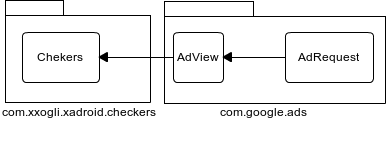
\includegraphics[scale=0.7]{pub}}
	      \end{center}
	\legend{Affichage de la publicité}
\end{figure}

\begin{table}[here]
    \begin{center}
	\begin{tabular}{|l|}
	\hline
	const/16 v1, 0x50 \\[0.2cm]
	
	invoke-virtual {v0, v1}, Lcom/google/ads/AdView;->setGravity(I)V \\[0.2cm]

	new-instance v1, Lcom/google/ads/AdRequest; \\[0.2cm]

	invoke-direct/range {v1 .. v1}, Lcom/google/ads/AdRequest;-><init>()V \\[0.2cm]

	invoke-virtual {v0, v1}, Lcom/google/ads/AdView;->loadAd(Lcom/google/ads/AdRequest;)V \\
	\hline
	\end{tabular}
    \end{center}
    \caption{\label{}code smali pour la publicité}
\end{table} 
La variable v1 contient l'instance de la classe \textit{com.google.ads.AdRequest} qui est le point d'entrée de la publicité dans l'application.
La variable v0 est la vue \textit{com.google.ads.AdView} associée à la publicité. Le chargement de la publicité ce fait par la méthode \textit{loadAd(AdRequest adrequest)}.


\appendix
\end{document}
